\setchapterimage{gears}
\chapter*{Application \arabic{cptApplication} \\ 
Détermination de l'inertie équivalente de réducteurs -- \ifprof Corrigé \else Sujet \fi}
\addcontentsline{toc}{section}{Application \arabic{cptApplication} : Détermination de l'inertie équivalente de réducteurs -- \ifprof Corrigé \else Sujet \fi}

\iflivret \stepcounter{cptApplication} \else
\ifprof  \stepcounter{cptApplication} \else \fi
\fi

%\setcounter{question}{0}
%\marginnote{Mines Ponts PSI -- 2003.}
%\marginnote[1cm]{
%\UPSTIcompetence[2]{B2-10}
%}
%\begin{marginfigure}
%\centering
%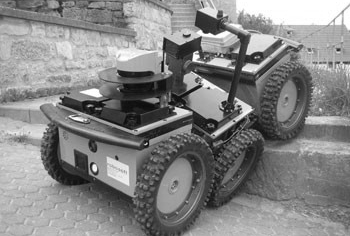
\includegraphics[width=4cm]{fig_00}
%\end{marginfigure}


\section*{Exercice 1 -- Calcul de l'inertie équivalente d'un train simple}

On donne un train d'engrenages simple avec $Z_1$, $Z_{21}$, $Z_{23}$ et $Z_3$ le nombre de dents des roues dentées. On nomme $k_1$ le rapport du train de $S_1$ et $S_2$ avec $k_1=\dfrac{\omega(2/0)}{\omega(1/0)}$ et  
$k_2$ le rapport de $S_2$ et $S_3$ avec $k_2=\dfrac{\omega(3/0)}{\omega(2/0)}$. 

On applique en entrée, sur l'arbre 1, un couple moteur $C_m\vect{z_0}$ destiné à entraîner une charge, sur l'arbre 3, modélisée par un couple résistant  $C_r\vect{z_0}$

\ifprof
\begin{center}
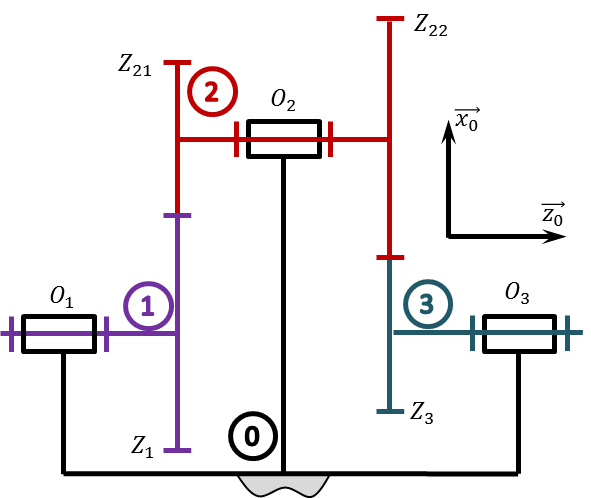
\includegraphics[width=.5\linewidth]{red_01}
\end{center}
\else
\begin{marginfigure}
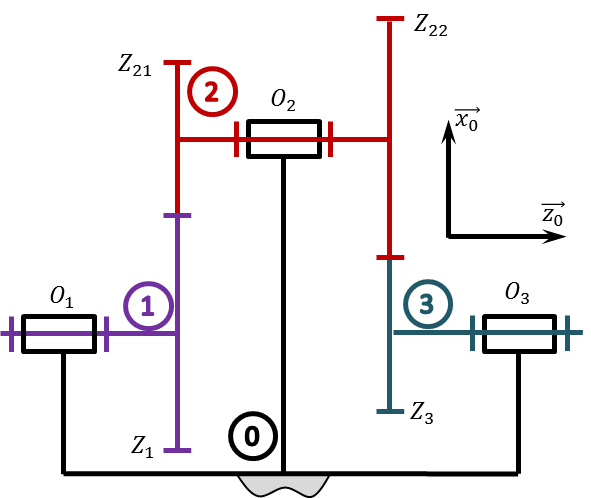
\includegraphics[width=\linewidth]{red_01}
\end{marginfigure}
\fi
On rappelle que pour les engrenages à denture droite $d=mz$ avec $d$ le diamètre primitif, $m$ le module, $z$ le nombre de dents du pignon. $\omega(1/0)$, $\omega(2/0)$ et $\omega(3/0)$ sont les vitesses de rotation de $S_1$, $S_2$ et $S_3$ autour des axes $\left(O_1,\vect{x_g}\right)$, $\left(O_2,\vect{x_g}\right)$ et $\left(O_3,\vect{x_g}\right)$. Le repère galiléen $\mathcal{R}_g$ est lié au solide $S_0$. Les liaisons pivots sont supposées parfaites. Les matrices d'inertie sont définies aux centres de masse $G_1=O_1$, $G_2=O_2$ et $G_3=O_3$ associées aux solides $S_1$, $S_2$ et $S_3$ sont de la forme : $\inertie{O_i}{S_i}=\matinertie{A_i}{B_i}{C_i}{0}{0}{0}{O_i,R_i}$.

Le train d'engrenage est entrainé par un couple moteur $C_m$ agissant sur la liaison pivot entre 1 et 0. Une charge résistante $C_r$ s'exerce sur l'arbre 3. 

\question{Déterminer le rapport de réduction du train d'engrenages.}

\question{Déterminer l'inertie équivalente du réducteur ramené à l'axe moteur.}

\question{Déterminer la relation entre le couple d'entrée et le couple de sortie du réducteur.}

\section*{Exercice 2 -- Calcul de l'inertie équivalente d'un train épicycloïdal}
%\setcounter{exo}{0}

On considère le train épicycloïdal suivant à trois satellites. Chacune des pièces est axisymétrique. On donne leurs matrices d'inertie :
$$
\overline{\overline{I_A}}(1) = 
\begin{pmatrix} 
A_1 & 0 & 0 \\
0 & B_1 & 0 \\
0 & 0 & C_1 \\
\end{pmatrix}_{\mathcal{R}_1}
\quad
\overline{\overline{I_B}}(2) = 
\begin{pmatrix} 
A_2 & 0 & 0 \\
0 & B_2 & 0 \\
0 & 0 & C_2 \\
\end{pmatrix}_{\mathcal{R}_2}
\quad
\overline{\overline{I_A}}(3) = 
\begin{pmatrix} 
A_3 & 0 & 0 \\
0 & B_3 & 0 \\
0 & 0 & C_3 \\
\end{pmatrix}_{\mathcal{R}_3}
$$


\begin{marginfigure}
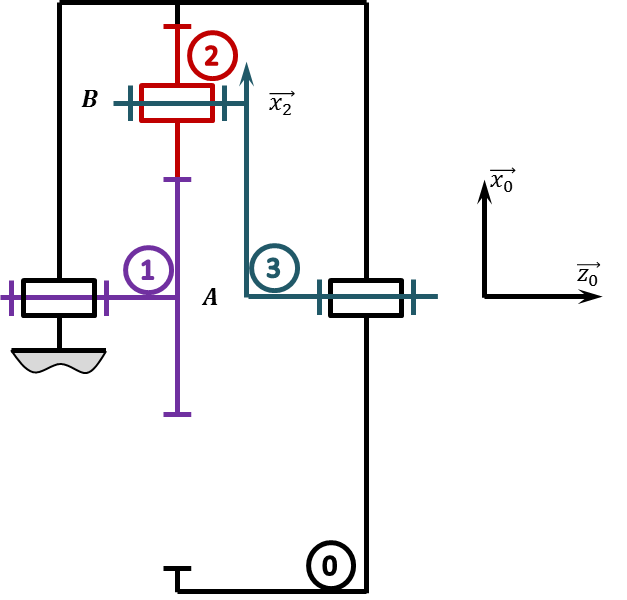
\includegraphics[width=\textwidth]{train_01}
\end{marginfigure}


On applique en entrée, sur l'arbre 1, un couple moteur $C_m\vect{z_0}$ destiné à entraîner une charge, sur l'arbre 3, modélisée par un couple résistant  $C_r\vect{z_0}$

%On montre que : $\mu = \dfrac{\omega(2/0)}{\omega(1/0)}=-\dfrac{r_1}{2r_2}$ .
\question{Déterminer le rapport de réduction du train épicycloïdal.}
\ifprof
\begin{corrige}
\begin{methode}
\begin{enumerate}
\item Écrire le rapport de réduction recherché.
\item Refaire le schéma en fixant le porte satellite et en libérant le bâti. Le porte satellite devient donc le bâti et le train peut être considéra comme un train simple.
\item Déterminer le rapport de réduction du train simple (les taux de rotation seront donc exprimés en fonction du porte-satellite) en fonction du nombre de dents des roues dentées.
\item Introduire les fréquences de rotation exprimées au point 1.
\item Exprimer le rapport de réduction cherché en fonction du  nombre de dents des solides. 
\end{enumerate}
\end{methode}


%\begin{minipage}[c]{.6\linewidth}
On recherche $k=\dfrac{\omega(3/0)}{\omega(1/0)}$. 

On bloque le porte satellite \textbf{3} et on libère la couronne \textbf{0}. 

On peut donc exprimer $ \dfrac{\omega(0/3)}{\omega(1/3)} = (-1)^1\dfrac{Z_1\cdot Z_2}{Z_2\cdot Z_0} = -\dfrac{Z_1}{Z_0}$.

En décomposant le taux de rotation, on introduit $\omega(1/0)$ et $\omega(0/3)$ :
$ \dfrac{\omega(0/3)}{\omega(1/3)} =  \dfrac{\omega(0/3)}{\omega(1/0)+\omega(0/3)} = -\dfrac{Z_1}{Z_0} 
\Leftrightarrow \dfrac{-\omega(3/0)}{\omega(1/0)-\omega(3/0)}  =-\dfrac{Z_1}{Z_0}  \Leftrightarrow {Z_0} \omega(3/0)  =Z_1 \left( \omega(1/0)-\omega(3/0)\right) 
\Leftrightarrow  \omega(3/0) \left(Z_0 + Z_1\right) =Z_1 \omega(1/0) 
\Leftrightarrow \dfrac{\omega(3/0)}{\omega(1/0)} = \dfrac{Z_1}{Z_1+Z_0}$.

Au final, $k = \dfrac{\omega(3/0)}{\omega(1/0)} = \dfrac{Z_1}{Z_1+Z_0}$.
%\end{minipage}\hfill
%\begin{minipage}[c]{.35\linewidth}
\begin{center}
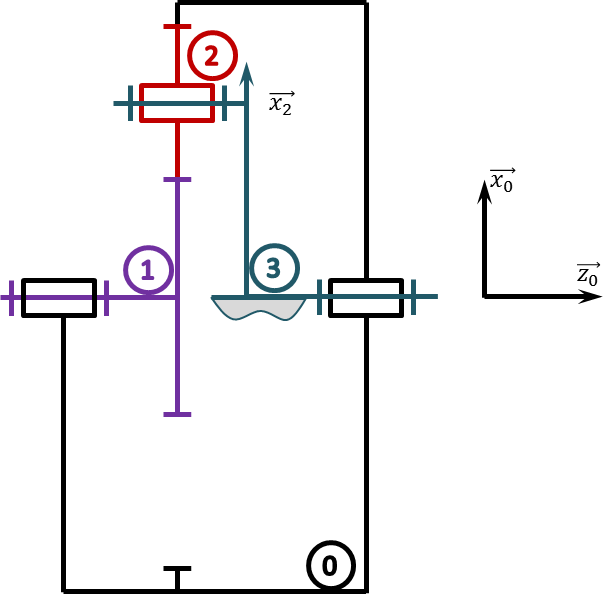
\includegraphics[width=\textwidth]{train_02}
\end{center}

%\end{minipage}
\end{corrige}
\else
\fi


\question{Déterminer l'inertie équivalente du train épicycloïdal.}


\question{Déterminer le couple moteur (à appliquer sur l'arbre 1) nécessaire à la mise en mouvement de la charge sur l'arbre de sortie 3 sur lequel est appliqué un couple résistant. }

%\subparagraph{}
%\textit{Déterminer l'énergie cinétique de l'ensemble $E=\{1,2,3\}$ par rapport au référentiel de la pièce \textbf{0} supposé galiléen.}
\ifprof
\begin{corrige}
\begin{methode}
\begin{enumerate}
\item On calcule $T(1/0)$, 
\end{enumerate}
\end{methode}
\textbf{Calcul de l'énergie cinétique du planétaire : $T(1/0)$}

Par définition, 
$2T(1/0)=\left\{\mathcal{V}(1/0) \right\} \otimes \left\{\mathcal{C}(1/0) \right\} $
$A$ étant un point fixe dans \textbf{0}, on a : 
$$
\left\{\mathcal{V}(1/0) \right\} = \torseurl{\vecto{1}{0}=\omega(1/0)\vect{z_0}}{\vectv{A}{1}{0}=\vect{0}}{A}$$

$$
\left\{\mathcal{C}(1/0) \right\} 
= \torseurl{M_1\vectv{G}{1}{0}}{\vect{\sigma \left( A\in 1/0\right)}=\overline{\overline{I}}\left( A,0\right) \vecto{1}{0}=C_1\omega(1/0)\vect{z}}{A}
$$
On a donc : 
$$T(1/0)=\dfrac{1}{2} C_1 \omega(1/0)^2 $$

\end{corrige}

\begin{corrige}
\textbf{Calcul de l'énergie cinétique du porte-satellite : $T(3/0)$}

Par définition, 
$2T(2/0)=\left\{\mathcal{V}(2/0) \right\} \otimes \left\{\mathcal{C}(2/0) \right\} $; on a : 
$$
\left\{\mathcal{V}(3/0) \right\} = \torseurl{\vecto{3}{0}=\omega(3/0)\vect{z_0}}{\vectv{A}{3}{0}=\vect{0}}{A}
$$

$$
\left\{\mathcal{C}(3/0) \right\} 
= \torseurl{M_3\vectv{G}{3}{0}}{\vect{\sigma \left( A\in 3/0\right)}=\overline{\overline{I}}\left( A,3\right) \vecto{3}{0}=C_3\omega(3/0)\vect{z}}{A}
$$
On a donc : 
$$T(3/0)=\dfrac{1}{2} C_3 \omega(3/0)^2=\dfrac{1}{2} k^2 C_3 \omega(1/0)^2 $$


\end{corrige}

\begin{corrige}

\textbf{Calcul de l'énergie cinétique d'un seul satellite : $T(2/0)$}

Par définition, 
$2T(2/0)=\left\{\mathcal{V}(2/0) \right\} \otimes \left\{\mathcal{C}(2/0) \right\} $ et le centre d'inertie d'un porte satellite est au point $B$ on a donc : 
$$
\left\{\mathcal{V}(2/0) \right\} = \torseurl{\vecto{2}{0}=\omega(2/0)\vect{z_0}}{\vectv{B}{2}{0}}{B} 
$$

$$
\left\{\mathcal{C}(2/0) \right\} 
= \torseurl{M_2\vectv{G}{2}{0}}{\vect{\sigma \left( A\in 2/0\right)}=\overline{\overline{I}}\left( A,2\right) \vecto{2}{0}=C_2\omega(2/0)\vect{z}}{A}
$$

$\vectv{B}{2}{0}= \vectv{B}{2}{3} + \vectv{B}{3}{0} = \vect{0}  + \vectv{A}{3}{0} + \vect{BA} \wedge \vecto{3}{0} = -R_3 \vect{x_3} \wedge \omega(3/0) \vect{z_0}= -R_3\omega(3/0)\vect{y_3} $.

\begin{rem}
Le vecteur $\vect{AB}$ est porté par le porte satellite. Par ailleurs, les points $A$, $B$ ainsi que les points de contact dans les engrenages sont toujours suivant la direction du porte satellite. 
Enfin, $R_3=R_1+R_2$.
\end{rem}
D'où : 
$$
\left\{\mathcal{V}(2/0) \right\} = \torseurl{\vecto{2}{0}=\omega(2/0)\vect{z_0}}{\vectv{B}{2}{0}=-R_3\omega(3/0)\vect{y_3}}{B}  
$$

$$\left\{\mathcal{C}(2/0) \right\} 
= \torseurl{M_2\vectv{G}{2}{0}=-R_3\omega(3/0)\vect{y_3}}{\vect{\sigma \left( A\in 2/0\right)}=C_2\omega(2/0)\vect{z}}{A}
$$

On a donc : 
$$T(3/0)=\dfrac{1}{2} C_2 \omega(2/0)^2 + \dfrac{1}{2}M_2 R_3^2 \omega(3/0)^2 
= \dfrac{1}{2} C_2 \dfrac{r_1^2}{4r_2^2}\omega(1/0)^2 + \dfrac{1}{2}M_2 R_3^2 k^2 \omega(1/0)^2
=\dfrac{1}{2} C_2 \mu^2\omega(1/0)^2 + \dfrac{1}{2}M_2 R_3^2 \omega(3/0)^2 
 $$


\end{corrige}

\begin{corrige}

\textbf{Calcul de l'énergie cinétique de l'ensemble E: $T(E/0)$}

Sans oublier qu'il y a 3 satellites (...), on a donc :
$$T(E/0)=T(1/0)+T(2/0)+T(3/0) $$

$$T(E/0) = \dfrac{3}{2} C_2 \dfrac{r_1^2}{4r_2^2}\omega(1/0)^2 + \dfrac{3}{2}M_2 R_3^2 k^2 \omega(1/0)^2 + \dfrac{1}{2} C_1 \omega(1/0)^2 + \dfrac{1}{2} k^2 C_3 \omega(1/0)^2
$$
D'où 
$$T(E/0) = \dfrac{1}{2}\left( 3 C_2 \mu^2 + 3M_2 R_3^2 k^2 + C_1  +  k^2 C_3 \right)\omega(1/0)^2
$$

On note donc $J_{eq} = 3 C_2 \mu^2 + 3M_2 R_3^2 k^2 + C_1  +  k^2 C_3$ l'inertie équivalente du train épicycloïdal.
\end{corrige}
%
%\begin{corrige}
%\begin{methode}
%\end{methode}
%\end{corrige}

\begin{corrige}
\textbf{Calcul des puissances externes}

\textbf{Calcul des puissances dues aux actions de contact}

\textbf{Puissance dissipée dans la liaison pivot entre 1 et 0 : $\mathcal{P}_{0\rightarrow 1}$ :} 


On a : $\mathcal{P}_{0\rightarrow 1} = \torseurcin{V}{1}{0} \otimes \torseurstat{T}{1}{0}$
$$
\torseurcin{V}{1}{0} 
= \torseurl{\vecto{1}{0}=\omega(1/0)\vect{z_0}}{\vectv{A}{1}{0}=\vect{0}}{A}  
\quad 
\torseurstat{T}{1}{0}
= \torseurl{\vectf{1}{0}}{\vectm{A}{1}{0}=L_{01}\vect{x_0} + L_{01}\vect{y_0}}{A}  
$$

On a donc : $\mathcal{P}_{0\rightarrow 1} = 0$.

\begin{itemize}
\item \textbf{Puissance dissipée dans la liaison engrenage entre 2 et 0 : $\mathcal{P}_{0\rightarrow 2}=0$ } 
\item \textbf{Puissance dissipée dans la liaison pivot entre 3 et 0 : $\mathcal{P}_{0\rightarrow 3}=0$ } 
\item \textbf{Puissance fournie à l'arbre 1 : $\mathcal{P}_{\text{ext} \rightarrow 1} = C_e \omega(1/0)$} 
\item \textbf{Puissance transmise par l'arbre 3 : $\mathcal{P}_{\text{3} \rightarrow \text{ext}} = C_s \omega(3/0) = k C_s \omega(1/0) $} 
\item \textbf{Calcul des puissances dues aux actions à distance}

\item \textbf{Puissance due à la pesanteur sur la pièce 1}

\item \textbf{Puissance due à la pesanteur sur la pièce 3}

\item \textbf{Puissance due à la pesanteur sur la pièce 2}

\item \textbf{Calcul des puissances internes}

\item \textbf{Puissance dissipée dans la liaison engrenage entre 1 et 2 : $\mathcal{P}_{1\rightarrow 2} = 0$ (RSG)} 


\item \textbf{Puissance dissipée dans la liaison pivot entre 2 et 3 : $\mathcal{P}_{3\rightarrow 2} = 0$}

D'après le théorème de l'énergie puissance, on a : 
$$
\dfrac{\text{d}T\left(E/0\right)}{\text{d}t} = \left( C_e + kC_s\right)\omega(1/0)
\Leftrightarrow
J_{eq}\dot{\omega}(1/0) = \left( C_e + kC_s\right)
$$
\end{itemize} 
\end{corrige}

\else
\fi